\section{Definition of Mixing}


There are a number of ways in which to define mixing. A fully 'mixed' solution is referred to, in this document, as when some solvent and solute combination have merged until the resulting solution has a consistent concentration of both. A consistent concentration is defined as the case when the number of solvent particles and solute particles in a sample volume taken from the solution is equal to the number in any other randomly chosen sample volume from the solution. This is the same as saying the probability of finding a solvent particle in a small volume is constant for the whole solution for any small volume of equal size.

However the definition of the verb 'mixing' is more ambiguous since it is the process via which the solvent and solute become mixed which is more difficult to quantify than detecting if a solution is 'fully mixed' which has a binary answer. In this specific project, the solution in question is dye in water being stirred by the three actuators. The mixing capability of each actuator will be explored by measuring the rate at which the dye is combined with the water using a number of different methods. These methods include inspecting the entropy of the mixture (Section~\ref{sec:entropy}), analysing fluid behaviour using PIV (Section~\ref{sec:PIV}) and modelling the dye-water mixture as a probability distribution (Section~\ref{sec:prob}). Effectively each method becomes a definition or quantifier for the rate of mixing and therefore mixing capability of each actuator.




\section{Initial Processing of Videos}
\label{sec:process}

As mentioned in Section~\ref{sec:Introduction}, the source videos show the mixing of dye and water using the three different sizes of actuator. Using certain analytical techniques such as Particle Image Velocimetry (explained further in Section~\ref{sec:PIV}), it is then possible to extract information from the system and use that to analyse and draw conclusions about the actuator and its efficiency.

Before they can be analysed, there is a lot of information the videos contain that can be seen as ineffectual. Each video contains 300 frames where each frame has an x coordinate (between 1 and 640), a y coordinate (between 1 and 480) and each pixel has different values for its Red, Green and Blue (RGB) components. This leads to approximately $2.76\times10^{8}$ values for each video. It is necessary to dimensionally reduce the information to make it manageable.


\subsection{Manipulating RGB Values}
\label{sec:rgb}

Since the dye within the tank is blue, looking at manipulating the RGB values is a way of reducing the dimensions and isolating the most relevant information. As each pixel in a frame has three values, one for red, green and blue, splitting these up allows for the same image to be analysed, but some of the superfluous data to be removed and ignored. 

%Can we show an image with the red, green and blue separately here?

\begin{figure}[H]
	\centering
	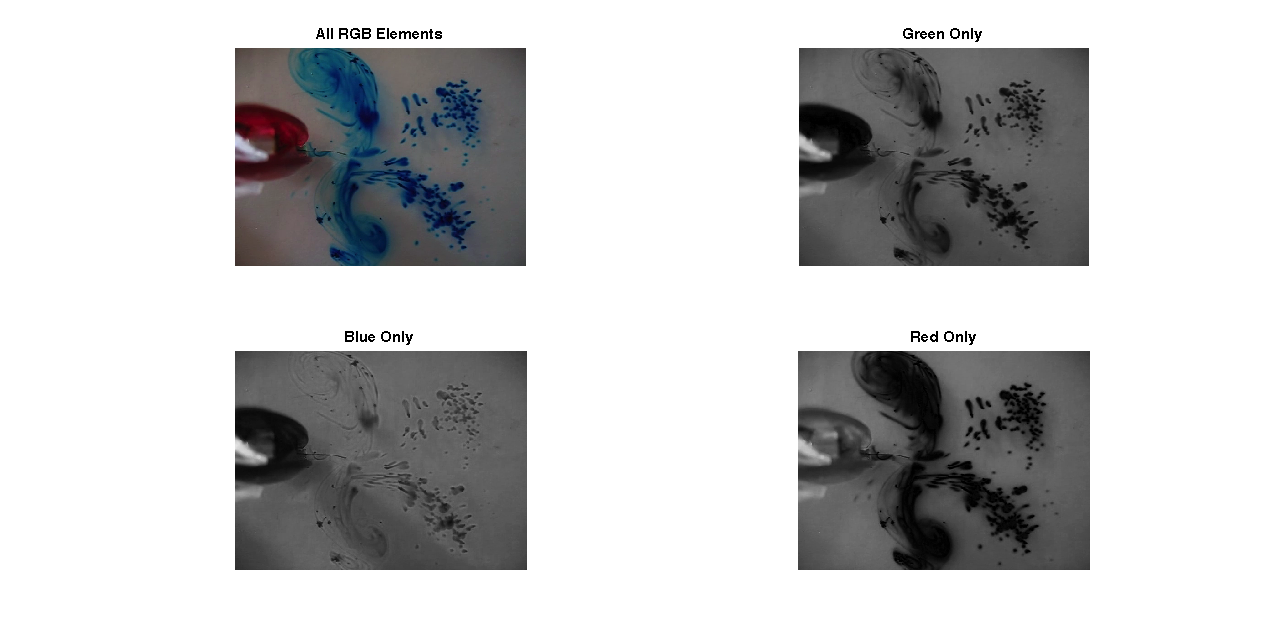
\includegraphics[width=1\textwidth]{Pictures/rgbshow.png}
    \caption{The original frame, 200, of the small actuator video and its red, green and blue components shown in greyscale.}
    \label{fig:rgbshow}
\end{figure}

%Yes

After splitting the frames into three different matrices, it is possible to show the matrices as images made up only of the values of the components of RGB, as can be seen in Figure~\ref{fig:rgbshow}.

The red values provide the best contrast due to the absence of red where the dye is concentrated.


\subsection{Using a Threshold Value}
\label{sec:threshold}

Another method of reducing the dimensionality of an image, to make it easier to process, is to set a threshold value. Threshold values cut out part of the image if the value for that pixel is either higher or lower than the value assigned. 

%Anything above 60 is cut from the image to clear it up
%Image of the distribution of values to show where the cut off is

\begin{figure}[H]
	\centering
	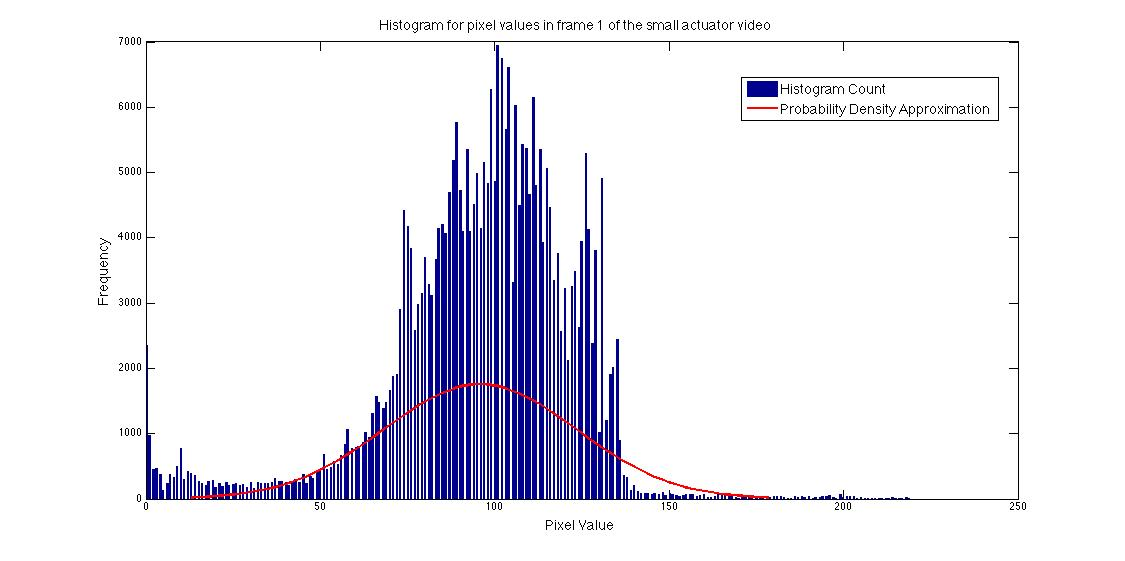
\includegraphics[width=1\textwidth]{Pictures/Pixel_Distribution.jpg}
    \caption{A histogram showing the distribution of the values for each pixel in frame 1, with a red filter, from the small actuator video. The threshold value was taken to be the bottom tenth percentile of this distribution. }
    \label{fig:pixeldistribution}
\end{figure}




The threshold value for these images was chosen to be 60 and anything higher was removed, meaning that only the darker points of the image were left. This was chosen because it is the 10th percentile of the values within the image, as seen in Figure~\ref{fig:pixeldistribution}. This means that any intensely white values were removed, and it left a clear space around the detail in the image, therefore any information about the dye in the water can be picked out more easily.

\begin{figure}[H]
	\centering
	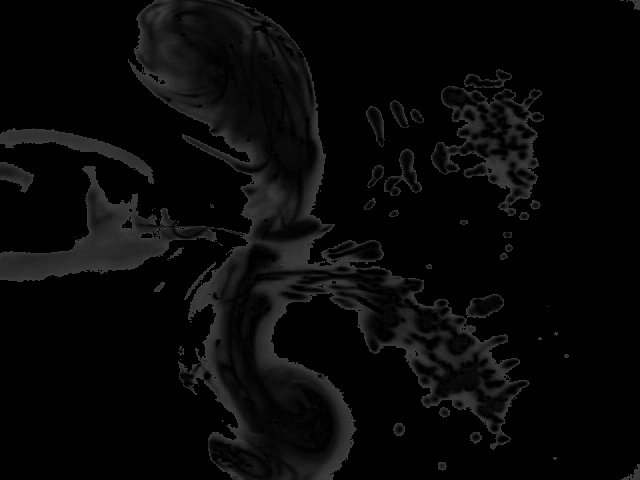
\includegraphics[width=0.6\textwidth]{Pictures/smallthresh.png}
    \caption{Image showing frame 200 in the small video with a red filter and threshold value of 60 applied; values above 60 are set to 0. }
    \label{fig:smallthresh}
\end{figure}




\subsection{Removing the Oscillator Mounting}
\label{sec:oscillatormountingremoval}

One element of the image that causes irregularities within the data is the actuator and its housing. As removing the oscillator from the image is a much more difficult subject in itself (see Section~\ref{sec:actuatortracking}), the main focus here is to remove the stationary housing that holds the oscillator in place. 
\newline

This is done by adding a black box on top of the oscillator mounting of zero values, meaning that values from that area would not be counted in any of the data analysis. This is the method used for two of the videos, the large and the medium, whereas for the small, because there is too much going on directly around the oscillator mounting area, three boxes were added to more efficiently mask the housing without removing any areas containing dye.

\subsection{Using the Complement}



Another way of reducing the noise that is within the image and focus on the concentration of dye, instead of using the threshold value, is to use the RGB images and to remove different components of the RGB from the others, for example blue minus green minus red.

\begin{figure}[h]

	\subfigure[Blue minus red minus green.]{
		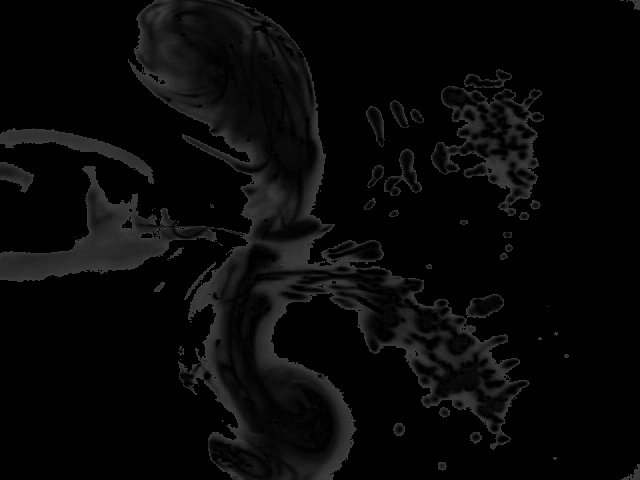
\includegraphics[width=\textheight/3]{Pictures/smallbrg.png} \label{fig:b-r-g}}
	\subfigure[Complement of blue minus red minus green.]{
		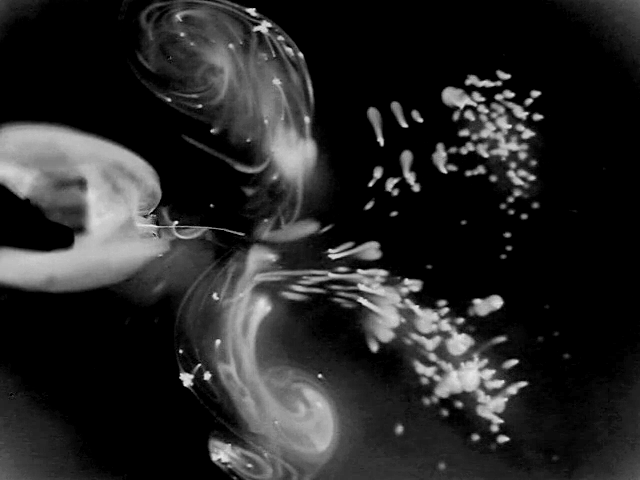
\includegraphics[width=\textheight/3]{Pictures/smallcbrg.png} \label{fig:cb-r-g}}
     \caption{Images of the blue minus red minus green, and the complement of blue minus the unchanged red minus the unchanged green, of frame 200 of the small video. The differences can be seen with the more intensely white parts of (b) showing up as black in (a).}
     
\end{figure}

As can be seen from Figure \ref{fig:b-r-g}, the areas with the intense blue are shown as black rather than white. This is because, in the original image, the red, green and blue values for these points are low. This means the red and green values negated the blue value to 0 (i.e. black).

In order to produce an image that shows the darker areas of blue dye as white rather than black, the complement of the blue provided the desired image. This means that when the red and green are taken away from it, the background is completely black and the intense blue areas in the original image are shown as white rather than black, such as in Figure \ref{fig:cb-r-g}. From this, and with the actuator housing removed, any non-zeros in the matrix can be taken to represent dye concentration.



\section{Actuator tracking and analysis}
\label{sec:actuatortracking}
A challenge in this project is the analysis of the actuators motion. Custom image processing techniques have been designed and are implemented to isolate the parts of the videos that represent the actuator.

The method description that follows is valid for the large actuator video, due to the relatively high number of pixels that make up the width of the actuator, as compared to the medium and small ones. The other two have insufficient data (pixels) representing the actuator to be able to extract useful information and produce reliable results. The process itself, however, is perfectly valid for an arbitrary actuator, provided that the video resolution is high enough. Therefore, the following section should be viewed as explanation of method using the large actuator as an example of usage, rather than as a presentation of numerical results.

\subsection{Process description}
First of all, the videos are manually trimmed, such that only the range of movement of the actuator is visible.

Subsequently, simple colour filtering is performed on video frames to maximise the visual difference between the actuator rod and the rest of the frame. Experimentally, it's been found that using the blue-only matrix gives best contrast for the isolation of the rod. Also, this reduces the dimensionality of the data: instead of using 3 matrices to represent each frame, only 1 is now required.

This results in pixels being represented by a value of blue only. The amount of blue in the pixel ranges from 0 (absence of blue which produces black in greyscale) to 255 (the highest intensity of blue which produces white in greyscale). The next step in processing the image is choosing a threshold which allows for the best isolation of the actuator. This is set at 60 (as discussed in Section~\ref{sec:threshold}), then any pixel with a value smaller than or equal to 60 is regarded as black, and all higher-value pixels are regarded as white. The process results in turning a numerical matrix into a logical one. This has an advantage in that the memory required to store the data is reduced from 8 bytes to just 1 byte per pixel \cite{matlab}, which speeds up the operations performed.


While the previous step largely removes the dye due to higher intensity of blue, some frames still have more concentrated regions of dye in them and appear as black. These are often disconnected from the actuator. By using a custom algorithm to pick out only the pixels in the frame which, when connected, make up a rod-like structure, the actuator is isolated. Figure \ref{fig:rodFiltering} shows an example of the method working on frame 117 of the large video.

\begin{figure}[h]

	\subfigure[Image of actuator after threshold is applied to blue value matrix.]{
\setlength{\fboxsep}{0pt}%
\setlength{\fboxrule}{1pt}%
\fbox{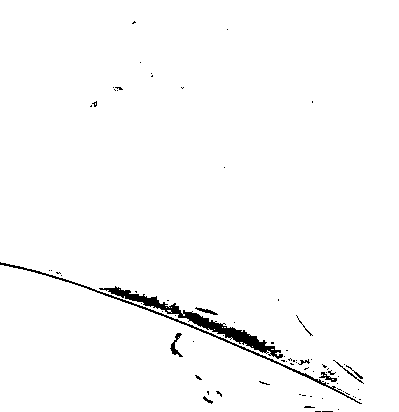
\includegraphics[width=\textheight/3]{Pictures/BW117.png}}}
	\subfigure[Final image after applying the filtering algorithm.]{
\setlength{\fboxsep}{0pt}%
\setlength{\fboxrule}{1pt}%
\fbox{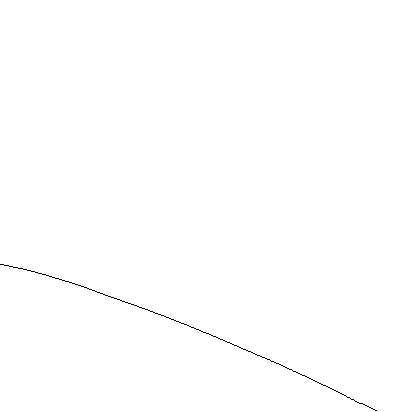
\includegraphics[width=\textheight/3]{Pictures/OnePixel117.png}}}

     \caption{Comparison of actuator images at different stages of filtering on frame 117.}
     \label{fig:rodFiltering}
     
\end{figure}


\subsection{Actuator reconstruction model}
In some frames of the video when the actuator is moving, the focus is lost and the frame becomes blurred. The fastest-moving parts, i.e. the furthest from the centre, are blurred enough to fall outside the [0, 60] range for blue values. Picking a higher cut-off threshold does not improve the detection, as too much of the dye is then present, making further algorithms obsolete.

To account for this, a model is developed, allowing the cut-off actuator parts to be reconstructed. 

For the majority of the frames, the actuator is moving slowly and its entire length is present after filtering and threshold value cut-off. For those where the movement is fast, about two-thirds of the length is still visible. This is enough to be able to extrapolate the shape of the actuator to its full length, based on the visible section detected. 

After final processing, each frame is represented by a matrix of 1’s and 0’s, such that there is only one black pixel per column of the frame. The x and y positions of 0’s have been used as data points in order to find a line of best fit. 

Through visual inspection, and through testing of various functions, including exponential, polynomial, and periodic functions over short intervals, a polynomial function is chosen and can be used to realistically extrapolate the shape of the actuator outside of the data points without overshooting. Degree n=3 has been chosen to represent the actuator’s shape due to a number of reasons:
\begin{enumerate}
  	\item	In a large number of frames, the shape of the actuator is a straight line. In these cases, the higher-order terms will be close to 0.
  	\item	For n=2, the general shape is preserved and is close to the original, but in some cases there is an offset between actual pixels and extrapolated ones, such that there is a gap in the shape. Further analysis of these frames shows that adding an extra degree to the polynomial will remove the offset - although the highest-degree term will only be small to account for the small fluctuations.
	\item	The modelling needs to be done only for the cases where a portion of the image is lost during the filtering phase. In these cases, about two-thirds of the shape is preserved.  The degree n=3 allows for a good degree of accuracy in data fitting, while extrapolation of the shape outside of the data points is still possible. This would not be possible with n=5, for example, as the y-values would rapidly grow.
	
\end{enumerate}	

Now the shape of the actuator in each frame varies and so the coefficients of the polynomial are different across the video. Therefore, a new polynomial of degree n=3 is found for each of the frames, and evaluated at subsequent points outside the original pixels range, until the point where the arc length of the new curve is equal to the arc length in frame 1 (since the picture in frame 1 is clear and filtered without loss of pixels).

Another method to reconstruct the shape is to evaluate the function up until the total number of 0's in the frame is the same as the starting frame (rather than comparing arclengths). There is no noticable difference between the two methods, and for further steps the arclength comparison is used.

\subsection{Motion analysis}

Taking the actuator analysis a step further, its motion is looked at in more detail. 

Four points along the length of the actuator are considered in the process of tracking its movements. They mark the beginning and the end of the rod, as well as two more points equally spaced in between, such that they are distributed at 1/3 and 2/3 of the length respectively. 

The y-positions of the points are plotted against the frame number to give Figure \ref{fig:pointsAlong}.

\begin{figure}[H]
	\centering
	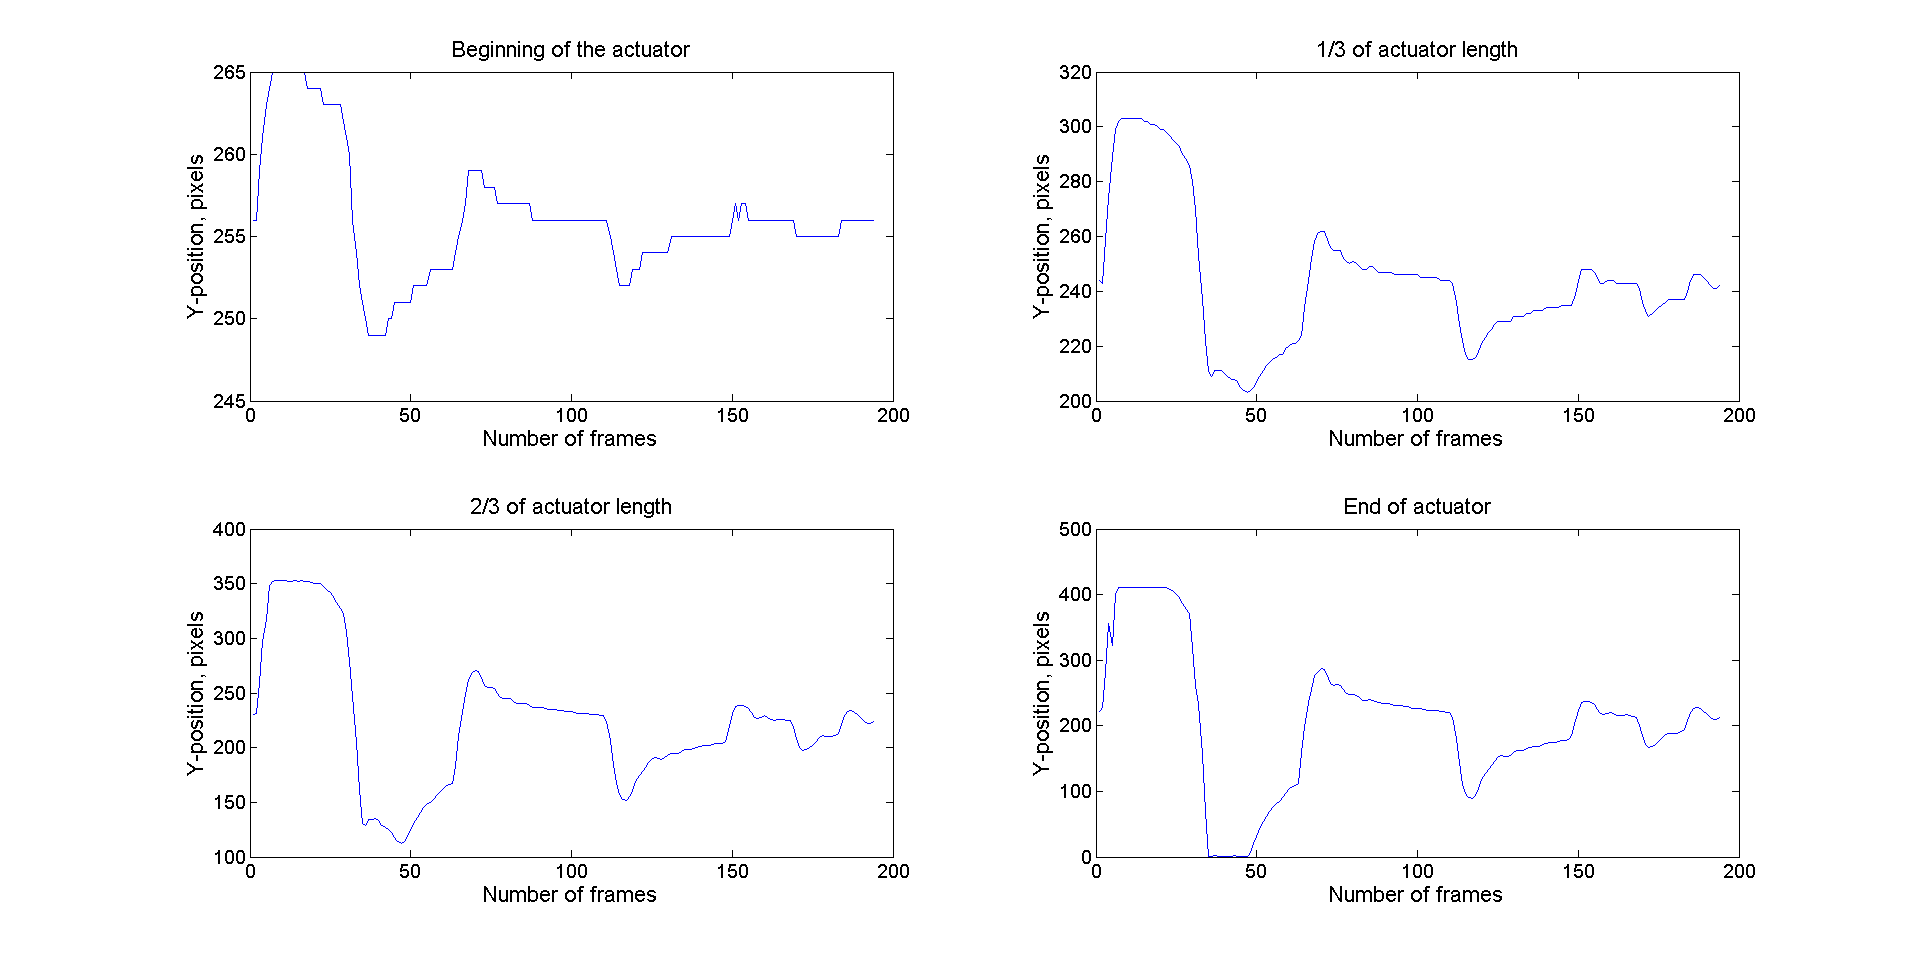
\includegraphics[width=1\textwidth]{Pictures/pointsAlongActuator.png}
     \caption{Plot showing how the y-position of pixels making up different points along the actuator varies with time.}
     \label{fig:pointsAlong}
\end{figure}

As expected, the general shape of the graph is the same for each four points, that is, their y-value starts increasing at the same time. The amplitudes of the jumps vary for the four reference points. The amplitude difference increases as the points move further down the length due to the bending motion of the actuator. From the graph, it can be deduced that for the duration of the video, the actuator performs 7 up/down movements in total; just over three oscillations.

It is expected that the initial section of the actuator would be stationary due to being fixed in the actuator housing however this is not the case in these results. An explanation for this is that in the initial stages of processing the video is trimmed. The real stationary part of actuator is cut out, since it is surrounded by its red casing, which makes further processing more complicated.

% To further examine the connection between amplitudes and position along the length of actuator, the max amplitude difference (here, as max(Amplitude) – min(Amplitude)) has been calculated for a all of the pixels that make up the image. This way, a clear relationship can be seen when the max amplitude difference is plotted against the position along the length:

% From the graph it can be seen that BLABLABLA

\subsection{Area calculation}

A useful application of actuator analysis is determining the area covered throughout its motion from which volume swept can be calculated. Both the number of frames (time intervals) and representation of the image are discrete values, so the equation for the total area swept is Equation \ref{eq:areaSum}:

\begin{equation}
	A_{total} = \sum_{i=1}^{N-1} |A_i - A_{i+1}|,
	\label{eq:areaSum}
\end{equation}


Where,
\newline
N = number of frames; \newline
$A_i$ = area under the curve at $i^{th}$ frame; 
\newline


The absolute value of the difference is calculated, to account for both directions of movement. Otherwise, the total area is zero (assuming the actuator returns to starting position).
This value is found to be 285361 pixels squared for the large actuator.

The volume can be found if the actuator width is known, however an important point to consider is that the number calculated only represents the volume covered by the actuator, not the total volume of liquid moved. This is due to fluid being pushed by actuator, but also pulled in by the effect of suction, which is created by regions of lower pressure as actuator pushes away. Also, the actuator transfers its energy into the fluid, which will give it momentum and the fluid circulates around the actuator in multiple directions, not just that of the actuator motion. Vortices are created, which are discussed in more detail in Section \ref{sec:vortices} of the report.




\section{Entropy as a Measure of Mixing}
\label{sec:entropy}
In general entropy is defined as a measure or quantifier of disorder, relating to the number of ways a system or message can be arranged. Since mixing can be described as increasing the disorder of a solvent-solute combination until a solution with maximum disorder - ie consistent concentration - is reached, entropy can be used as a measure for how well mixed a solution is.

In order to assess the mixing efficiency of the given actuators, it is necessary to find some way of measuring entropy from the video frames. Image-entropy is used for this. The entropy of an image is a measure of the 'business' in the image, sometimes used in image compression algorithms since it relates to the amount of information coding required in order to completely describe the image in question. If there is little activity and low contrast in a frame it will have low image-entropy. 

This measure of entropy is calculated for all pixels in a frame using Equation~\ref{eq:entropy} where $p_i$ is the probability that the difference between two adjacent pixels in an image is equal to $i$.

\begin{equation}\label{eq:entropy}
Entropy = -\sum\limits_{i}^{}p_{i}\log_2 p_{i}
\end{equation}

In MATLAB, the values of entropy for every frame of the three videos were calculated demonstrating the change in system entropy over time as shown in Figure~\ref{fig:entplot}. All three videos have a marked increase in entropy at the time of initial actuator movement (shown by dashed lines), with image-entropy continuing to increase over time. As described previously the entropy of a solution with consistent concentration would theoretically be zero. However, as the dye is spread around the frame from concentrated areas during the mixing the entropy will actually increase before eventually reducing to 'zero' as the solution becomes fully mixed. In the results, the increase in entropy demonstrates the rate of initial mixing, however the state of being well mixed is never reached in the videos so no final decrease in entropy is observed.

A number of sudden jumps are observable in the magnitude of entropy at seemingly random points over time. Analysis of this concluded that these are in most part caused by changes in exposure or by sudden appearance of shadows in the videos. It is also unreasonable to directly compare the entropy values between each actuator since the scattering, quantity and intensity of the dye in the water, as well as the exposure, vary between the videos, which directly affect the entropy measure. 

While it seems that conclusive information cannot be reliably drawn from these results, they do show a similar increasing trend in the entropy of each of the three systems. The 112 and 117 actuator systems in particular have similar results with a sharp initial increase in entropy that then reduces over time as the actuator oscillations decrease in frequency and amplitude. This is expected since the first oscillation of each actuator has the greatest amplitude and transfers more energy to the fluid than later oscillations. The 1110 actuator is not only powered with more energy than the two smaller systems (by a factor of 40) but also, due to its scale, much of the dye solution is swept out of frame by the actuator. The results are therefore expected to be different for this system in comparison to the others, which is evident.


\begin{figure}[H]
	\centering
	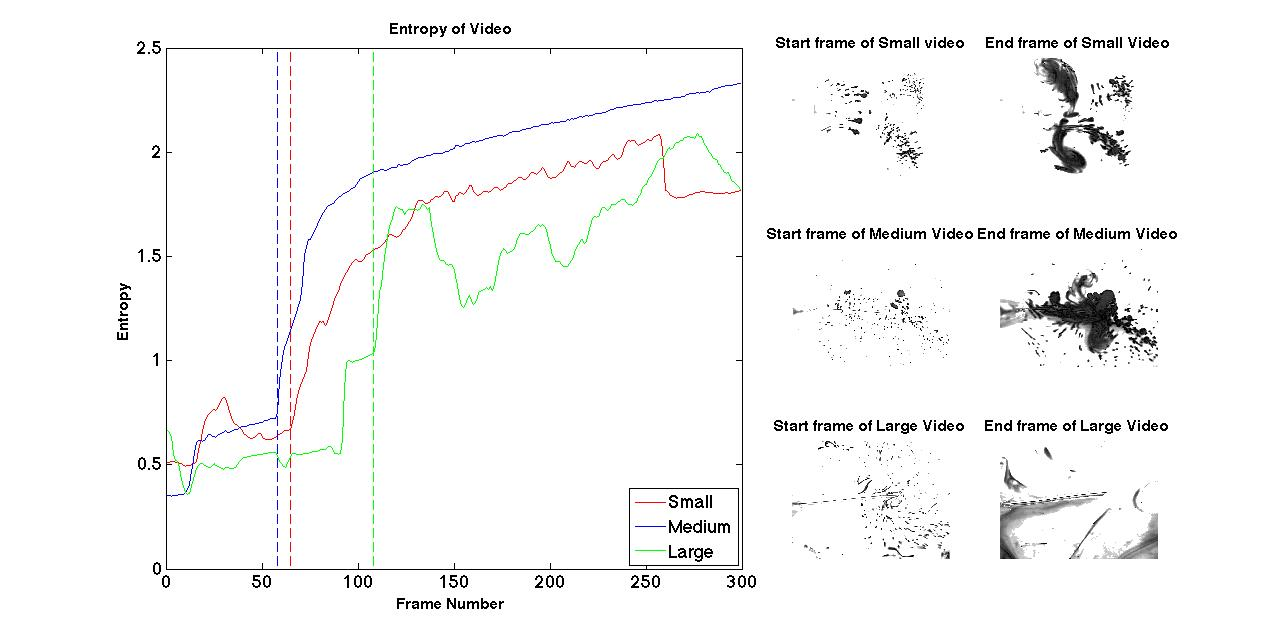
\includegraphics[width=1\textwidth]{Pictures/entropyplot.jpg}
    \caption{Plot of the image entropy value calculated using Equation~\ref{eq:entropy} for every frame in each of the three videos. Actuators 112 (Small), 117 (Medium) and 1110 (Large). Vertical dashed lines refer to the frame in which  motion of each actuator begins. Initial and final frames are shown (right) for each actuator demonstrating processing (red filtering and threshold) applied prior to calculating entropy.}
    \label{fig:entplot}
\end{figure}



\begin{figure}[H]
	\subfigure[112 actuator]{
	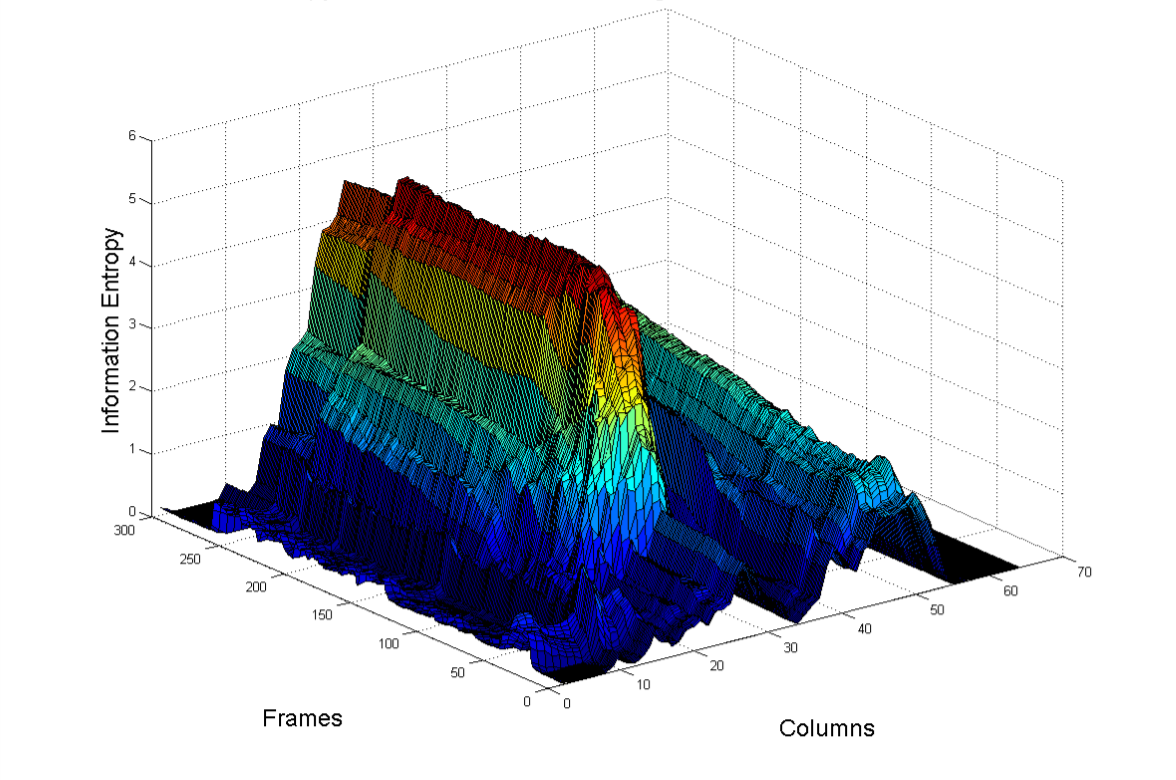
\includegraphics[width=0.45\textwidth]{Pictures/EntDistSmall.png}}
	\subfigure[117 actuator]{
	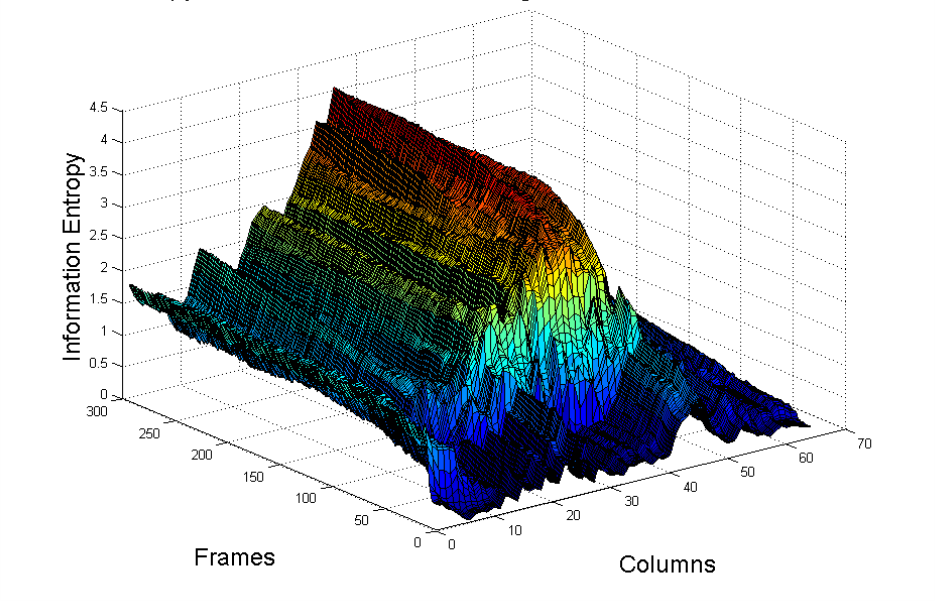
\includegraphics[width=0.45\textwidth]{Pictures/EntDistMed.png}}
    \center
	\subfigure[1110 actuator]{
	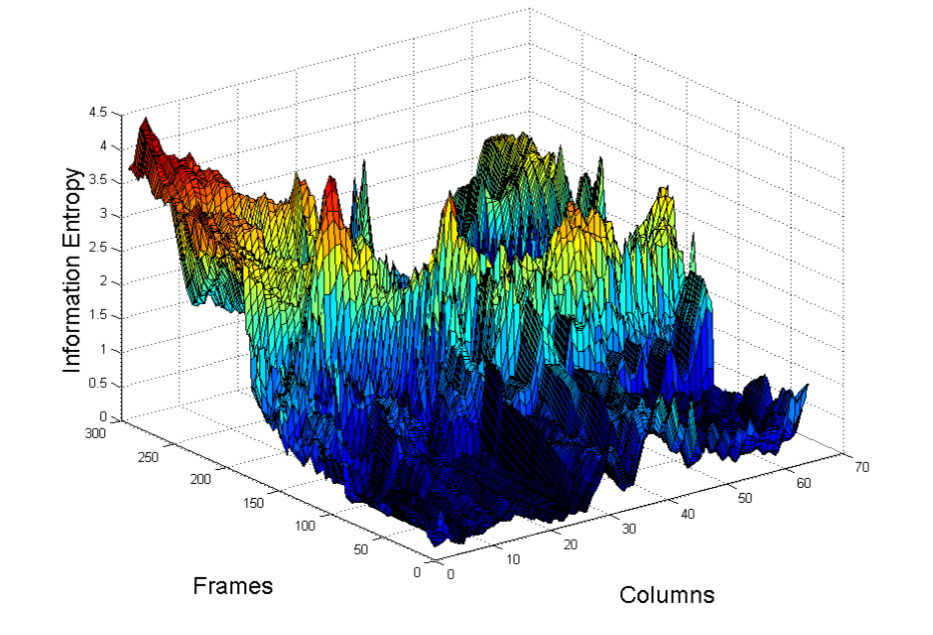
\includegraphics[width=0.45\textwidth]{Pictures/EntDistLarge.png}}
     \caption{3D entropy plot over time using the entropy of vertical sections of each frame.}
     \label{fig:entplots}
\end{figure}


Expanding upon this to get a more informed visual view of the change in entropy over time for each system,  the video frames are split into columns with 10 pixel width. Image entropy is then calculated for each column within the frame so that a vector containing entropy values is associated with each frame. Plotting these entropy distributions for all frames in the video gives a 3D plot for each actuator displaying the horizontal entropy distribution over time. These are shown in Figure~\ref{fig:entplots} for each actuator.


From these plots it is much clearer to see how the entropy is distributed across each frame. All three start with roughly uniform low entropy as the the dye is localised in concentrated areas across the image. Once the voltage is applied to the actuators, the mixing of the dye creates more 'activity' in the frame and the entropy increases rapidly, mostly in the central region for 112 and 117 where the majority of mixing occurs. The 1110 actuator has a very different plot since the actuator fills a large portion of the frame and sweeps some of the dye out of the picture. 


If the actuator experiment was to be repeated, the filming could include the entire container of liquid being mixed and a different method for applying voltage used that induces a continuous motion of the actuators. The filming could continue for the length of time it takes for the solution to be as close to fully mixed as is achievable. In addition, if identical lighting conditions are used for each video and identical scattering of dye, then image-entropy could be conclusively used as a measure of the rate of mixing for each actuator. The most efficient actuator could then be determined by noting the length of time before the image-entropy falls below some threshold indicating a well-mixed solution, shorter time indicating a faster rate of mixing.
  



\section{Particle Image Velocimetry}
\label{sec:PIV}

%http://pivlab.blogspot.de/

%Definition of PIV?

From the three videos given, it is possible to visualise the flow and velocity of the fluid over time in a two dimensional vector field. Although a vector field will provide more information on what is happening within the fluid, it may not provide quantitative information for analysis. Particle Image Velocimetry (PIV) is a method of image analysis which provides a vector field with quantitative values at each point.

There are many forms of PIV which require different components and different types of computational analysis. Accurate and reliable PIV tests use two cameras focused on a single point, a light source (laser) to illuminate the region of interest (usually in the form of a plane) and tracer particles that can be clearly identified and tracked. The videos produced from the experiments did not include tracer particles or a laser light source. However, it is still possible to use PIV using a method called Cross Correlation.

Cross Correlation uses small sub spaces of the image called interrogation areas. These interrogation areas are compared between two frames in chronological order and use the Discrete Cross-Correlation function (Equation \ref{eq:crosscorr})\cite{flappybird} to find the particle pattern in the same interrogation area for two frames.

 \begin{equation}\label{eq:crosscorr}
 C(m,n)=\sum_{i}\sum_{j}A(i,j)B(i-m,j-n)
 \end{equation}
where A and B are the same interrogation areas from image A and B.

The matrix C that is produced from Equation \ref{eq:crosscorr} gives what can be called the agreement between A and B for a given shift. In essence, the matrix produced contains peaks where the interrogation area in A is most similar to B given the shift $(m,n)$ in coordinates. The maximum peak value given within the matrix C at $C(m,n)$ tells us that the most probable match of A to B is from the coordinate shift $(m,n)$ and that is the most probable displacement of the particle. This process is repeated for interrogation areas across the images and then produces a vector field such that each centre of the interrogation area has a velocity value associated with it. It can be noted that having larger interrogation values will increase the signal to noise ratio of the cross correlation. However, increasing the interrogation area will decrease the resolution of the velocity vector field. Table \ref{table:vecres} shows the effect of changing the interrogation area on an image with resolution 240x240 pixels.
\begin{table}[H]
\begin{center}
\begin{tabular}{| c | c| }
	\hline
    Interrorgation Area & Vector Field Resolution \\
    \hline
    120x120 & 2x2\\
    \hline
    10x10 & 24x24\\
    \hline
    4x4 & 60x60\\
    \hline
    2x2 & 120x120\\
    \hline

\end{tabular}
\caption{For an image with resolution 240x240, the effect on the resolution of the vector field with the change of the size of the interrogation area}
\label{table:vecres}
\end{center}
\end{table}
Calculating this for all 300 frames is computationally intense in the spatial domain. This is known as Direct Cross-Correlation (DCC). The computational strain this causes can be overcome by producing the cross-correlation in the frequency domain by applying a Fourier Transform known as 'Fastest Fourier Transform in the West'(FFTW) which is a software technique that optimises speed for Fourier Transformations \cite{fftw3}. Using the frequency domain does have its disadvantages when in use. Every particle displacement causes loss of information, which is produced in the form of background noise for the cross-correlation matrix. Also, FFTW assumes the interrogation areas are periodic (and repeat themselves in all directions). This means that a displacement that is larger than half the size of the interrogation area will be incorrectly mapped.

In order to justify the use of Cross-Correlation PIV with FFTW mapping, a few assumptions are made. The first one being that the size of the particles on the screen are large enough to be resolvable in the footage and remain that size throughout. It is true that the dye does not act as a single particle in water, but this assumption allows the use of PIV. The second assumption is that the frame rate is fast enough such that the particles are not moving greater than half the distance of the interrogation area between each frame. This assumption allows the use of FFTW since the computer systems used may not have been powerful enough to handle a DCC analysis.

After these assumptions are made and the program used (PIVlab \cite{pivlab}) has been set up, it is then possible to use the pre-processed frames using the Red value (explained in Section \ref{sec:rgb}) and the threshold limit (explained in Section \ref{sec:threshold}) and produce a vector field of each video at each frame.

The settings used to analyse and produce the vector field were that the FFTW was used instead of the DCC. This allowed less computational strain on the computer that was used. Each frame was triple passed with varying interrogation areas. The first pass had an interrogation area of 64x32, the second pass interrogation area was 32x16 and the final third pass was 16x8. The reason a triple pass was used to allow each pass to compare results with the previous passes. As mentioned above, higher interrogation areas yield a better signal to noise ratio, yet decrease the vector field resolution. Allowing a combination of larger and smaller interrogation areas allows the resulting vector field to have the highest resolution (the third pass) that takes into account the information gained from the previous passes (first and second).

\begin{figure}[H]
\centering
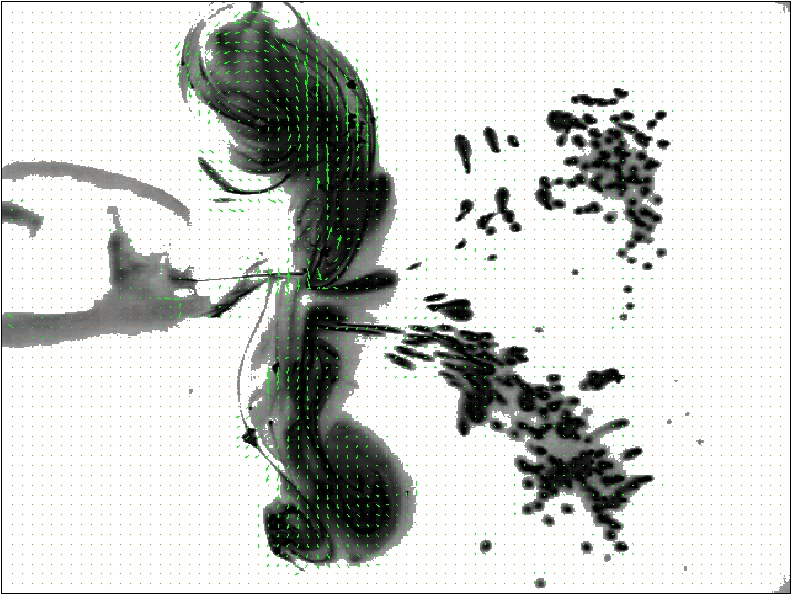
\includegraphics[width=0.6\textwidth]{Pictures/PIVlab_out_small_110_110.jpg}
     \caption{The vector field produced by the PIV analysis of the smallest actuator at the 110th frame including the 110th frame after red filter and threshold applied.}
     \label{fig:PIVfield}
\end{figure}

Seen in Figure \ref{fig:PIVfield}, the vector field produced can qualitively show how the particles move over time. PIV also produces quantative values of the velocity of the fluid which can then be used to look at the curvature of the field (explained in Section \ref{sec:vortices}). It should be noted that the results given are as accurate as the video used and the assumptions used can be refined and changed to produce more accurate results.


%(ref: http://tejas.serc.iisc.ernet.in/currsci/jul102000/review%20article.pdf)

%PIV for different filters/thresholds?

%Images of the PIV in action?

%What can be found?

%What is curl?


\section{Tracking Vortices using PIV}
\label{sec:vortices}


The Particle Image Velocimetry data produces a velocity vector field describing the motion of the fluid in every frame of the videos. This information is contained in individual matrices for each frame. The curl of a velocity vector field $\bar{F}$ (denoted as $curl \bar{F}$) describes the rotational tendency of all particles within the field as given in Equation~\ref{eq:curl}. In specific relation to the dye in the water, the curl of the velocity vector fields describes the circulation of the dye particles. Using curl, vortices can be detected by locating areas with sizeable and consistent rotation and their strength calculated. 


\begin{equation}\label{eq:curl}
curl \bar{F}= \bigtriangledown\times\bar{F} = \Bigg| \begin{matrix}
  	i & j & k \\
  	\frac{\partial}{\partial{x}} & \frac{\partial}{\partial{y}} & \frac{\partial}{\partial{z}} \\
  	\bar{F}_{x} & \bar{F}_{y} & \bar{F}_{z}
	\end{matrix} \Bigg|
\end{equation}

Figure~\ref{fig:curl1} shows the resulting curl plots for frames 50, 150, 250 of the 112 actuator video as a colormap underlayed beneath the relevant PIV vector fields. The colour is scaled according to the range of values in the frame, so varies between frames. All points for which velocity is zero have zero curl and the colour at these points represents neutral fluid motion. Warm colours (red, orange) represent clockwise rotation in the fluid, cool colours (blue, cyan) represent anti-clockwise rotation. These plots are the clearest result from experimenting with interrogation size and magnifying features within the PIV data. Even with this, the vortices and overall fluid motion is not clear using the given videos and detecting sizeable vortices is only successful for frames in the region 100-150. The resulting curl plots for the 117 actuator are similar, however the 1110 actuator video has no detectable vortices and the curl plots are less clear.

An example of successful vortex detection in frame 150 is shown in Figure~\ref{fig:curl2}. 


\begin{figure}[H]

	\subfigure[Frame 50]{
		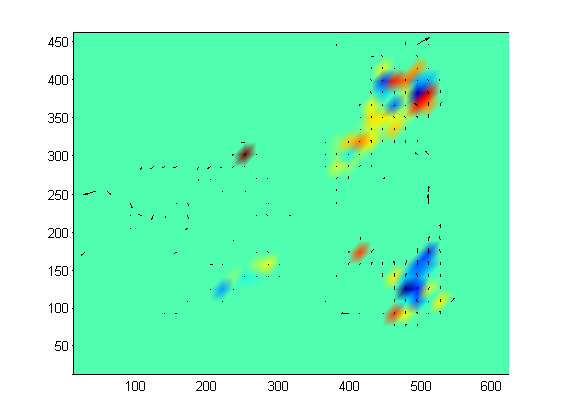
\includegraphics[width=\textheight/3]{Pictures/curlFrame50.png}}
	\subfigure[Frame 150]{
		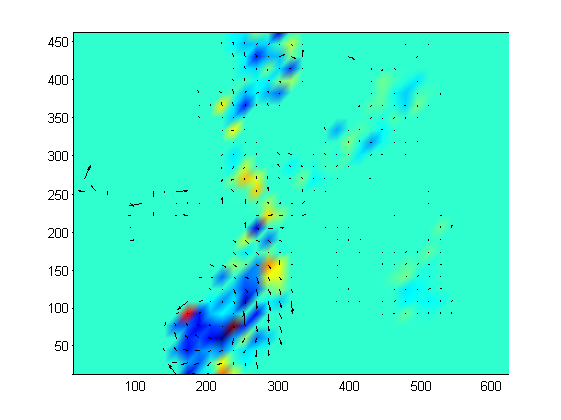
\includegraphics[width=\textheight/3]{Pictures/curlFrame150.png}}
	\center
  	\subfigure[Frame 250]{
  		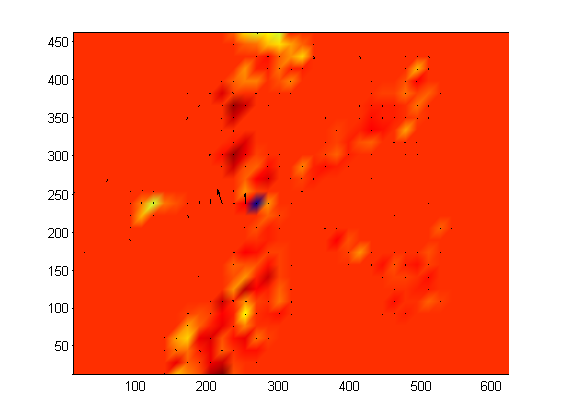
\includegraphics[width=\textheight/3]{Pictures/curlFrame250.png}}

   
     \caption{Showing the PIV vector field with underlayed curl colormap for different frames of the 112 actuator video.}
      \label{fig:curl1}
     
\end{figure}

\subsection{Curl Plot Analysis}

A fully mixed solution would be expected to have zero curl since the velocity vector field would be zero due to the lack of detectable movement in a fluid of consistent concentration. However, in relation to the specific videos being analysed, the state of consistent concentration is not reached and it can be conjectured as to which detected motion in the fluid is demonstrative of most efficient mixing. The fluid behaviour expected for ideal mixing will be some combination of high speed particles with changing direction, however there are infinite possibilities making it difficult to define ideal behaviour.

If a greater difference in velocity of neighbouring particles increases the rate of mixing then the conclusion can be drawn that multiple strong vortices of alternating direction in the fluid would have the best mixing action. However, this form of mixing, in effect inducing turbulent behaviour of the fluid\cite{curl}, has fast movement and mixing of particles local to vortices but overall mixing is not as efficient. Fewer vortices with large radii would cause greater displacement of particles across the overall frame but dye in the centre would be recirculated within the same local area and also not mixing efficiently with the rest of the solution. 

Simulating multiple situations of fluid flow and comparing the rate of mixing for each falls outside the time scope for this project, therefore the assumption is made that increased momentum of the fluid results in increased mixing rate, disregarding the number of vortices as well as their direction and location. Fluid momentum can be calculated once the strengths of vortices are known. Extrapolating this to find the momentum of all vortices in the wake of the actuator can be used as a measure of mixing efficiency, since greater momentum of fluid in the wake is assumed to increase the rate of mixing.

As mentioned the video data available does not provide suitable curl plots to be able to detect clear vortices across the wake so calculating an accurate result for the total momentum is not feasible. If data with conclusive results from vortex detection is available, then the method for calculating fluid momentum is outlined in Section~\ref{sec:momentum}.

 

\begin{figure}[H]
     
     \center
     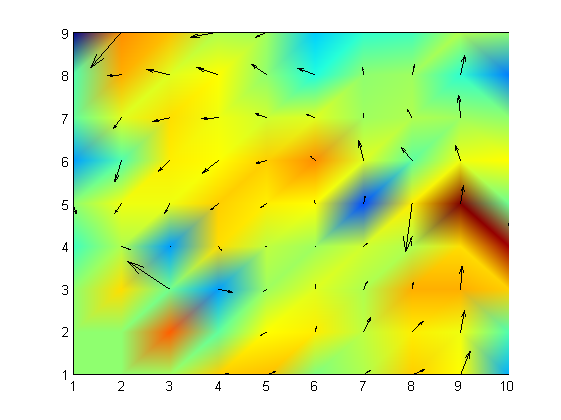
\includegraphics[width=0.4\textheight]{Pictures/newCurl.png}
     \caption{Subsection of frame 150 for the 112 actuator video focusing on the largest detected vortex with center (210, 80).}
     \label{fig:curl2}
\end{figure}

\subsection{Method for calculating fluid momentum}
\label{sec:momentum}
 

The strength of an ideal vortex can also be defined as the circulation $\Gamma$ of the vortex. The circulation can be calculated by taking the line integral of the fluid velocity $\bar{V}$ tangential to the vortex about a chosen curve $C$ as given in Equation~\ref{eq:curl2}. 


\begin{equation}\label{eq:curl2}
\Gamma = \oint_{C} \bar{V} \,  \bar{dl}
\end{equation}

Here $\bar{dl}$ represents the path element vector for the line integral and $C$ is a closed curve encircling the vortex. This assumes that the tangential velocity is known for all points on the curve $C$ which is not the case since the given velocity vector field data is discrete values in a matrix. Therefore, before vortex strength can be calculated, the tangential velocity at all points on $C$ must be found by interpolating from the known values and taking the component tangential to $C$.


This calculation can be repeated for multiple circles $C$ of different radii in order to approximate the total circulation. For the planar section of a vortex within a wake such as that in Figure~\ref{fig:curl2}, the fluid momentum can then be calculated using the circulation, planar area $A$ and the fluid density $\rho$ using Equation~\ref{eq:curl3} \cite{swimmingfish}.


\begin{equation}\label{eq:curl3}
M= \rho \Gamma A
\end{equation}
 





\section{Modelling Systems as Probability Distributions}
\label{sec:prob}

By modelling each frame of the videos as a probability distribution, separate frames can be compared in relation to the rate of mixing using statistical tests. 

\subsection{Calculating Probability Distribution}

The frame data used for calculating the probability distribution is processed by taking the complement of each frame to reverse the colours and removing the green and red components as well as blocking out the actuator housing as described in Section~\ref{sec:process}.  This leaves a matrix that mostly contains zeros shown as black with higher values in greyscale representing the dye. The more concentrated the dye in an area is, the higher the values in that area of the matrix, shown as brighter areas of white in the frame.

With the frames in this format, any non-zero values can be used to represent particles of dye. A probability distribution is formed by finding the total sum of matrix values for every pixel or square interrogation area of the frame and dividing these by the total amount of dye in the frame. This gives the probability of finding dye particles in that section of the frame at that time. 

The probability distribution for frame 200 of each video is shown in Figure \ref{fig:probd} using a section size of 8x8 pixel squares across each frame.

\vspace{2cm}


\begin{figure}[H]
     

	\subfigure[112 actuator]{
		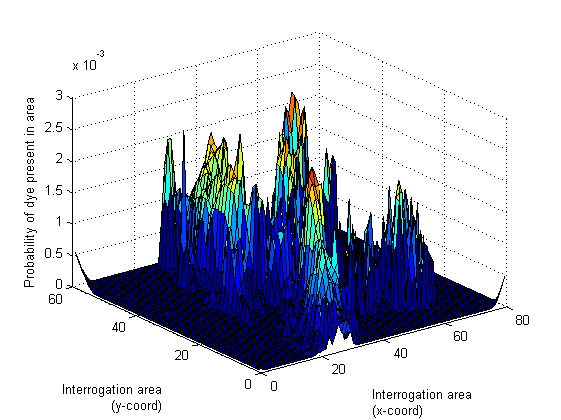
\includegraphics[width=0.5\textwidth]{Pictures/probDist1.png}}
	\subfigure[117 actuator]{
		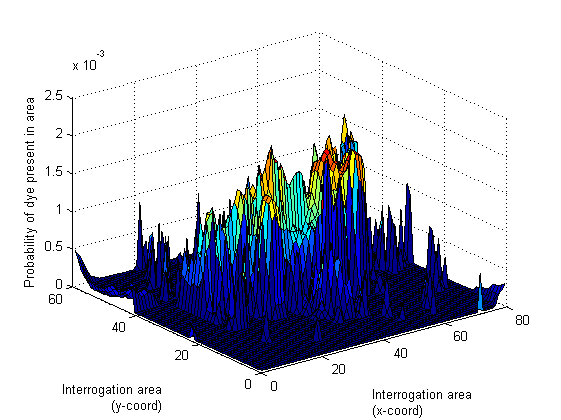
\includegraphics[width=0.5\textwidth]{Pictures/probDist2.png}}
    \center
	\subfigure[1110 actuator]{
		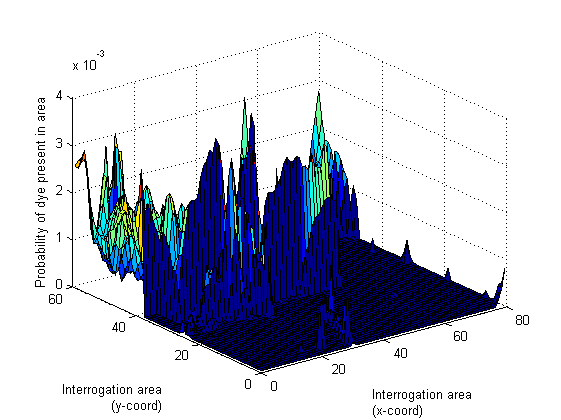
\includegraphics[width=0.5\textwidth]{Pictures/probDist3.png}}
  
     \caption{Visual plots of the probability distribution for frame 200 of each video.}
     
     \label{fig:probd}
\end{figure}



\subsection{Statistical Test Analysis}
By treating the data as a sample from some overall probability distribution that describes the system for each time interval, two frames can be compared by assessing the likelihood they are both samples from the distribution. In this instance the T-test is used with a null hypothesis that two sets of frame data are from the same overall probability distribution given a set significance level. Since the change is small between consecutive frames, it would be expected that they would have a high likelihood of being from the same distribution leading to the null hypothesis being accepted. Two frames many time intervals apart would lead to the null hypothesis being rejected. 

By comparing frames at different time intervals apart, the number of time intervals at which the null hypothesis is no longer accepted can be found. This time span is a measure of the rate at which the image is changing which is indicative of the rate at which the dye is being mixed in the water. If the actuator is mixing efficiently, a rapid change in the distribution of dye across the frame is expected leading to the rejection of the null hypothesis for frames close together in time.



\begin{figure}[H]
     \label{fig:ttest}

	\subfigure[112 actuator]{
		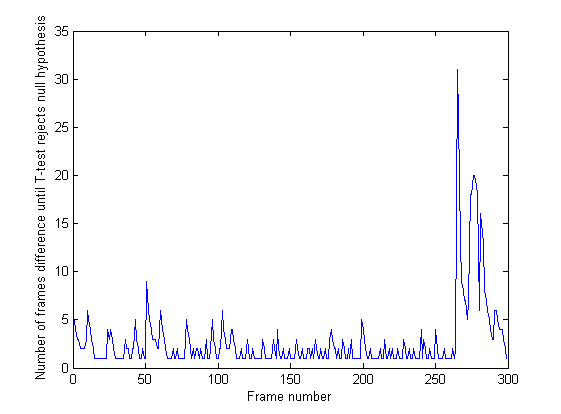
\includegraphics[width=\textheight/3]{Pictures/ttestpic1.png}}
	\subfigure[117 actuator]{
		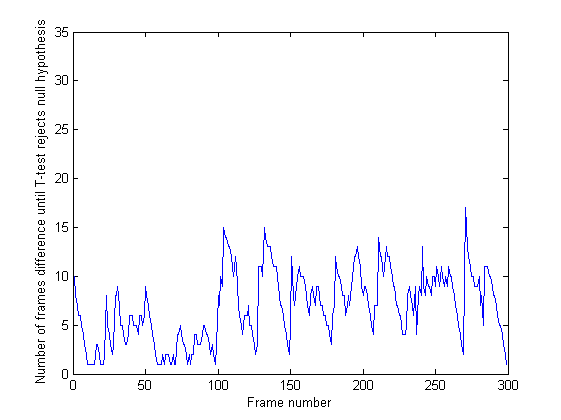
\includegraphics[width=\textheight/3]{Pictures/ttestpic2.png}}
    \center
	\subfigure[1110 actuator]{
		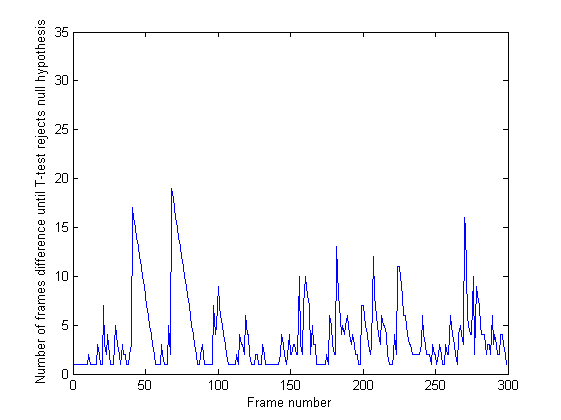
\includegraphics[width=\textheight/3]{Pictures/ttestpic3.png}}
  
     \caption{For each frame of the three videos a T-test is taken to compare the frame with subsequent frames as time increases until the T-test rejects the null hypothesis and returns 1. The graphs show the number of time intervals that occur until the frame at which the T-test returns 1 for each frame. }
    

\end{figure}


The results of using the T-test in reality do not show a clear universal result that can be used to indicate the mixing rate. The plot for the 112 actuator is closest to giving the expected result since the values in the range 100-270 are noticeably small - all under 5 - indicating that the data in the frame is rapidly changing. However there is no conclusive trend and comparison between all three actuators yields no conclusions. The test produces the same results when repeated while iterating over the frames backwards in time, verifying the method, but cannot be used to draw any conclusions about the mixing efficiency of the actuators.


\section{Conclusion}

The aim of the report was to analyse the footage of IPMC actuators mixing water and blue dye to determine information about the system. The key focus was to identify which size actuator produced the most consistently mixed solution. This was not conclusively determined for the given video data, however methods and measures to assess mixing efficiency have been described.

The reconstruction of the actuator would allow for a look into the energy used for movement. If the model could then be refined by looking at more data, it would help provide a more accurate description of the actuator's movement. The energy lost in transmission and other parts of the system could be analysed and show areas that need to be addressed.

Looking into quantifying mixing in terms of entropy was not reliable considering the data given. However, for a longer and more controlled recording of the mixing with the actuator oscillating for a greater period of time could be analysed for mixing efficiency using the method discussed. 

The probability distribution of certain interrogation areas of the frames can give a good quantification of mixing since a "well-mixed solution" converges to a uniform distribution. It was found, however, that using a statistical test to compare frames did not produce conclusive results in this instance.

The vector field produced by using PIV analysis is good for considering the movement of particles and having a first look into the curl and vortices produced but not enough to produce reliable data to analyse the fluid behaviour. In order for a more accurate representation of the flow of the fluid flow, the experiment would have to be repeated. It would be advisable to have a laser illuminating the plane of interest, two cameras focusing on a single point and a computer that will be able to handle the higher computational stresses of DCC. This would produce a more accurate vector field that could then be used for momentum calculations by inspecting detected vortices in the flow.  
